\documentclass[xcolor={usenames, dvipsnames}]{beamer}
\usepackage{amsmath, amssymb}
\usepackage[export]{adjustbox}
\usepackage{tikz}
\usepackage{wrapfig}
\usepackage{bm}
\usepackage{graphicx}

\mode<presentation> {
\usetheme{Singapore}
}

\title{\#1 Chad Allen Zhao gets the hottest girl in the grade}
\author{Ramesh Balaji, Duc Nguyen, Allen Zhao}
\date{June 11, 2021}

\begin{document}

\frame{\titlepage}

\begin{frame}
    The series was now tied 3-3, with game 7 determining the outcome of the series. 
    The game was a close one: Lebron kept flopping for fouls, Curry and Allen were 
    exchanging threes, while Tacko and Giannis fought for paint dominance. It all came 
    down to one final play. With the Lakers leading 144-143 with 12 seconds left in the 
    4th quarter, Giannis curled around an Anthony Davis screen and cut back door.
     Lebron drove down the right lane and floated up a lob perfectly placed in Giannis’ 
     strong hands. 
\end{frame}

\begin{frame}
    Allen anticipated this, and jumped up to block the dunk. Giannis'
    attempt was absolutely pummeled by Allen's block and he accelerated down the
    court for the fast break. He was striding up the right side of the court,
    like a giraffe through the savannah. Tacko zoomed up the left side, creating
    a 2 on 1 fast break opportunity, with only Lebron ahead of them.
\end{frame}
\begin{frame}
    As Allen handled the ball, he noticed Lebron gradually slowing down.
    \emph{He's going to flop and draw a charge,} Allen thought. With Tacko being open
    and ahead of him, Allen knew he had to snap a quick pass so that he could
    dunk it right before the clock struck 0 for the 145-144 win. Allen was a
    diligent star student in AP Calculus AB back in the day, and performed some
    quick maths in his head.
\end{frame}
\begin{frame}
    Naturally, he knew that he was $7 ft$ in front of half court, his
    current velocity was $14 \frac{ft}{s}$ forward, and that his running acceleration
    could be modeled by the function $a_{1}(t) = 0.5t^2 + 3$, in $\frac{ft}{s^2}$. 
    Glancing at Tacko, he observed that he was $23 ft$ to the left of him and $12 ft$ in
    front of half court. His current velocity was $18 \frac{ft}{s}$ up the court, and
    being Tacko's best friend, Allen was certain his acceleration was modeled by
    $a_2(t) = 0.6t^2 + 3$. Allen knew he'd have to zip a $51 \frac{ft}{s}$ dot straight at
    Tacko for him to catch it and dunk it on time. The only question is, what is the rate of 
    change of the angle between Allen and Tacko when Tacko (hopefully) catches the ball?
\end{frame}

\begin{frame}

\begin{center}

    \begin{figure}[t]
        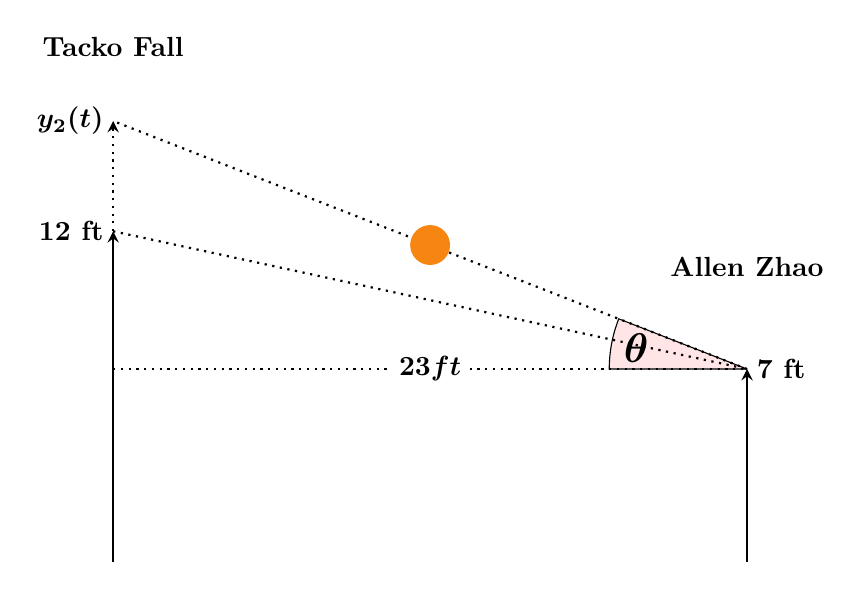
\begin{tikzpicture}[scale=0.35]
            \draw
                [fill=red!10] (23,1) 
                -- (18,1) arc[start angle=180, end angle=158.629,radius=5cm] 
                -- (23,1);
            \draw[->, >=stealth, thick] 
                (0,-6) -- (0, 6);
            \draw[->, >=stealth, thick][dotted] 
                (0, 6) -- (0, 10);
            \draw[->, >=stealth, thick] 
                (23, -6) -- (23,1);
            \draw[dotted, thick]
                (0,6) -- (23,1);
            \draw[dotted, thick]
                (0,1) -- (23,1);
            \draw[dotted, thick]
                (23,1) -- (0,10);
            \draw
                (23,1) node[anchor=west] {\textbf{7 ft}};
            \draw
                (0,6) node[anchor=east] {\textbf{12 ft}};
            \draw
                (0,10) node[anchor=east] {\bm{$y_{2}(t)$}};
            \draw
                (18,1.75) node[anchor=west][scale=1.5] {\bm{$\theta$}};
            \draw 
                (0,12) node[anchor=south] {\textbf{Tacko Fall}};
            \draw 
                (23,4) node[anchor=south] {\textbf{Allen Zhao}};
            \node[fill=white] at (11.5,1) {\bm{$23 ft$}};
            \filldraw[color=BurntOrange] 
                (11.5, 5.5) circle (20pt);
        \end{tikzpicture}
    \end{figure}
    
\end{center}

\end{frame}

\begin{frame}

    \centering

    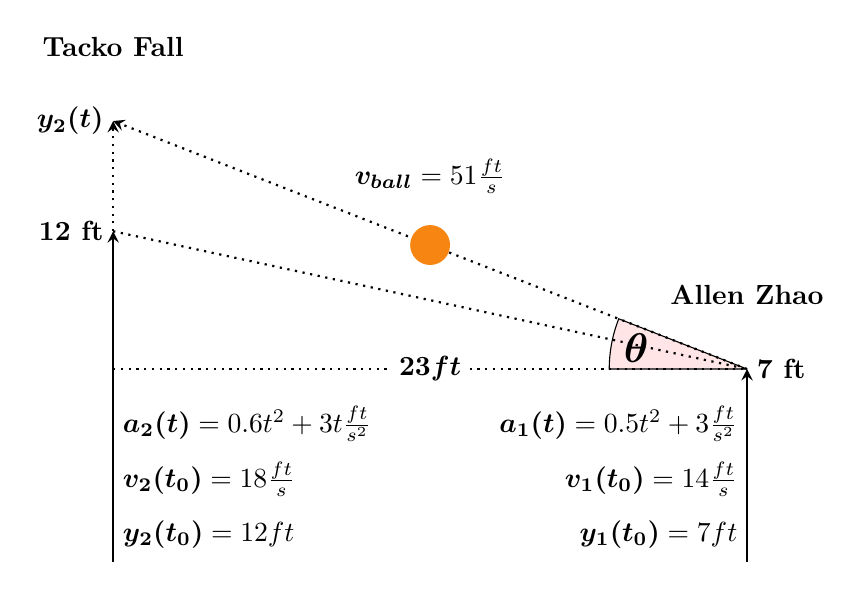
\begin{tikzpicture}[scale=0.35]
        \draw[fill=red!10] (23,1) 
            -- (18,1) arc[start angle=180, end angle=158.629,radius=5cm] 
            -- (23,1);
        \draw[->, >=stealth, thick] (0,-6) -- (0, 6);
        \draw[->, >=stealth, thick][dotted] (0, 6) -- (0, 10);
        \draw[->, >=stealth, thick] (23, -6) -- (23,1);
        \draw[dotted, thick]
            (0,6) -- (23,1);
        \draw[dotted, thick]
            (0,1) -- (23,1);
        \draw[->, >=stealth, dotted, thick]
            (23,1) -- (0,10);
        \draw
            (23,1) node[anchor=west] {\textbf{7 ft}};

        \draw
            (0,6) node[anchor=east] {\textbf{12 ft}};
        \draw
            (0,10) node[anchor=east] {\bm{$y_{2}(t)$}};
        \draw
            (18,1.75) node[anchor=west][scale=1.5] {\bm{$\theta$}};
        \draw 
            (0,12) node[anchor=south] {\textbf{Tacko Fall}};
        \draw 
            (23,3) node[anchor=south] {\textbf{Allen Zhao}};
        \draw
            (0,-1) node[anchor=west] {$\bm{a_{2}(t)} = 0.6t^2+3t \frac{ft}{s^2}$};
        \draw
            (0,-3) node[anchor=west] {$\bm{v_{2}(t_{0})} = 18 \frac{ft}{s}$};
        \draw
            (0,-5) node[anchor=west] {$\bm{y_{2}(t_{0})} = 12ft$};
        \draw
            (23, -1) node[anchor=east] {$\bm{a_{1}(t)} = 0.5t^2 + 3 \frac{ft}{s^2}$};
            \draw
            (23, -3) node[anchor=east] {$\bm{v_{1}(t_0)} = 14 \frac{ft}{s}$};
        \draw 
            (23, -5) node[anchor=east] {$\bm{y_{1}(t_0)} = 7 ft$};
        \draw
            (11.5, 7) node[anchor=south] {$\bm{v_{ball}} = 51 \frac{ft}{s}$};
        \filldraw[color=BurntOrange] 
            (11.5, 5.5) circle (20pt);
        \node[fill=white] at (11.5,1) {\bm{$23 ft$}};
    \end{tikzpicture}\par

\end{frame}

\begin{frame}

    \centering

    \begin{figure}[t]
    
    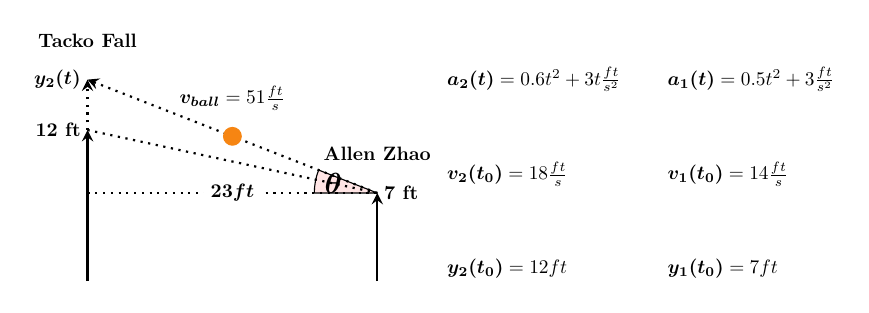
\begin{tikzpicture}[scale=0.16, every node/.style={scale=0.7}]
        \draw[fill=red!10] (23,1) 
            -- (18,1) arc[start angle=180, end angle=158.629,radius=5cm] 
            -- (23,1);
        \draw[->, >=stealth, thick] (0,-6) -- (0, 6);
        \draw[->, >=stealth, thick][dotted] (0, 6) -- (0, 10);
        \draw[->, >=stealth, thick] (23, -6) -- (23,1);
        \draw[dotted, thick]
            (0,6) -- (23,1);
        \draw[dotted, thick]
            (0,1) -- (23,1);
        \draw[->, >=stealth, dotted, thick]
            (23,1) -- (0,10);
        \draw
            (23,1) node[anchor=west] {\textbf{7 ft}};

        \draw
            (0,6) node[anchor=east] {\textbf{12 ft}};
        \draw
            (0,10) node[anchor=east] {\bm{$y_{2}(t)$}};
        \draw
            (18,1.75) node[anchor=west][scale=1.5] {\bm{$\theta$}};
        \draw 
            (0,12) node[anchor=south] {\textbf{Tacko Fall}};
        \draw 
            (23,3) node[anchor=south] {\textbf{Allen Zhao}};
        \draw
            (28,10) node[anchor=west] {$\bm{a_{2}(t)} = 0.6t^2+3t \frac{ft}{s^2}$};
        \draw
            (28,2.5) node[anchor=west] {$\bm{v_{2}(t_{0})} = 18 \frac{ft}{s}$};
        \draw
            (28,-5) node[anchor=west] {$\bm{y_{2}(t_{0})} = 12ft$};
        \draw
            (45.5, 10) node[anchor=west] {$\bm{a_{1}(t)} = 0.5t^2 + 3 \frac{ft}{s^2}$};
        \draw
            (45.5, 2.5) node[anchor=west] {$\bm{v_{1}(t_0)} = 14 \frac{ft}{s}$};
        \draw 
            (45.5, -5) node[anchor=west] {$\bm{y_{1}(t_0)} = 7 ft$};
        \draw
            (11.5, 7) node[anchor=south] {$\bm{v_{ball}} = 51 \frac{ft}{s}$};
        \filldraw[color=BurntOrange] 
            (11.5, 5.5) circle (20pt);
        \node[fill=white] at (11.5,1) {\bm{$23 ft$}};
    \end{tikzpicture}\par

\end{figure}

Before Allen uses any of his given information on the motion of Fall and himself,
he should first look at the overarching equation for $\frac{d\theta}{dt}$.
    %
    \begin{align*}
        tan(\theta) &= \frac{(12ft-7ft) + \Delta y_{2} ft}{23 ft} \\
        \theta &= tan^{-1}(\frac{5 + \Delta y_{2}}{23}) \\
        \frac{d\theta}{dt} &= \frac{1}{23} \cdot \frac{1}{1 + (\frac{5 + \Delta y_{2}}{23})^2} \cdot \frac{d(5 + \Delta y_{2})}{dt}
    \end{align*}
    %
\end{frame}

\begin{frame}

    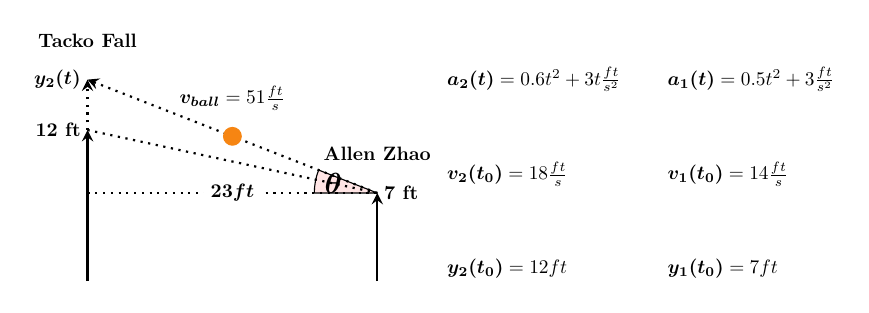
\begin{tikzpicture}[scale=0.16, every node/.style={scale=0.7}]
        \draw[fill=red!10] (23,1) 
            -- (18,1) arc[start angle=180, end angle=158.629,radius=5cm] 
            -- (23,1);
        \draw[->, >=stealth, thick] (0,-6) -- (0, 6);
        \draw[->, >=stealth, thick][dotted] (0, 6) -- (0, 10);
        \draw[->, >=stealth, thick] (23, -6) -- (23,1);
        \draw[dotted, thick]
            (0,6) -- (23,1);
        \draw[dotted, thick]
            (0,1) -- (23,1);
        \draw[->, >=stealth, dotted, thick]
            (23,1) -- (0,10);
        \draw
            (23,1) node[anchor=west] {\textbf{7 ft}};

        \draw
            (0,6) node[anchor=east] {\textbf{12 ft}};
        \draw
            (0,10) node[anchor=east] {\bm{$y_{2}(t)$}};
        \draw
            (18,1.75) node[anchor=west][scale=1.5] {\bm{$\theta$}};
        \draw 
            (0,12) node[anchor=south] {\textbf{Tacko Fall}};
        \draw 
            (23,3) node[anchor=south] {\textbf{Allen Zhao}};
        \draw
            (28,10) node[anchor=west] {$\bm{a_{2}(t)} = 0.6t^2+3t \frac{ft}{s^2}$};
        \draw
            (28,2.5) node[anchor=west] {$\bm{v_{2}(t_{0})} = 18 \frac{ft}{s}$};
        \draw
            (28,-5) node[anchor=west] {$\bm{y_{2}(t_{0})} = 12ft$};
        \draw
            (45.5, 10) node[anchor=west] {$\bm{a_{1}(t)} = 0.5t^2 + 3 \frac{ft}{s^2}$};
        \draw
            (45.5, 2.5) node[anchor=west] {$\bm{v_{1}(t_0)} = 14 \frac{ft}{s}$};
        \draw 
            (45.5, -5) node[anchor=west] {$\bm{y_{1}(t_0)} = 7 ft$};
        \draw
            (11.5, 7) node[anchor=south] {$\bm{v_{ball}} = 51 \frac{ft}{s}$};
        \filldraw[color=BurntOrange] 
            (11.5, 5.5) circle (20pt);
        \node[fill=white] at (11.5,1) {\bm{$23 ft$}};
    \end{tikzpicture}\par

    \begin{align*}
        \frac{d\theta}{dt} = \frac{1}{23} \cdot \frac{1}{1 + (\frac{5 + \Delta y_{2}}{23})^2} \cdot \frac{d(5 + \Delta y_{2})}{dt}
    \end{align*}
    %
    Now, we need to solve for $\Delta y_2$. To do that, we need the time ($t$) 
    it takes for the ball to travel to Fall's future position. By Pythagoras, 
    %
    \begin{align*}
        (51 \cdot t)^2 = 23^2 + (5+\Delta y_2)^2
    \end{align*}

\end{frame}

\begin{frame}

    \begin{figure}[t]
        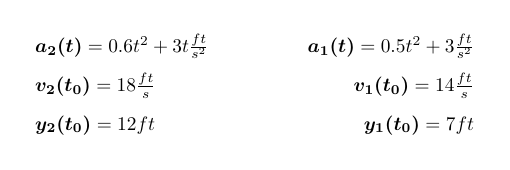
\begin{tikzpicture}[scale=0.25, every node/.style={scale=0.7}]
            \draw
                (0,-1) node[anchor=west] {$\bm{a_{2}(t)} = 0.6t^2+3t \frac{ft}{s^2}$};
            \draw
                (0,-3) node[anchor=west] {$\bm{v_{2}(t_{0})} = 18 \frac{ft}{s}$};
            \draw
                (0,-5) node[anchor=west] {$\bm{y_{2}(t_{0})} = 12ft$};
            \draw
                (23, -1) node[anchor=east] {$\bm{a_{1}(t)} = 0.5t^2 + 3 \frac{ft}{s^2}$};
            \draw
                (23, -3) node[anchor=east] {$\bm{v_{1}(t_0)} = 14 \frac{ft}{s}$};
            \draw 
                (23, -5) node[anchor=east] {$\bm{y_{1}(t_0)} = 7 ft$};
        \end{tikzpicture}
    \end{figure}

    Let's solve for $\Delta y_2$ and $t$. To do this, we will need to integrate $a_2(t)$, 
    then $v_2(t)$ given the initial positions and velocities. 
    %
    \begin{align*}
       (51 \cdot t)^2 -23^2 &=(5+\Delta y_2)^2 \\
       \sqrt{(51 \cdot t)^2 - 23^2} - 5 &= \Delta y_2\\
       \int_{0}^{t} (18\frac{ft}{s}+\int_{0}^{t} (0.6t^2+3t) \ dt) \ dt &= \Delta y_2 \\
       \int_{0}^{t} (18\frac{ft}{s}+\int_{0}^{t} (0.6t^2+3t) \ dt) \ dt &= \sqrt{(51 \cdot t)^2 - 23^2} - 5 \\
       t = 0.535 s, \Delta y_2 &= 9.718 ft
    \end{align*}

\end{frame}

\begin{frame}

    Now, we can finally solve for $\frac{d\theta}{dt}$. 
    $\frac{d(5+\Delta y_2)}{dt}$ would be the sum of Tacko's inital velocity and 
    the accumulation due to his acceleration $0.535$ s in the future:
    %
    \begin{align*}
        18\frac{ft}{s}+\int_{0}^{0.535}(0.6t^2+3t) \ dt = 18.461 \frac{ft}{s}
    \end{align*}
    %
    \begin{center}
        With everything plugged in:
    \end{center}
    %
    \begin{align*}
        \frac{d\theta}{dt} &= \frac{1}{23} \cdot \frac{1}{1 + (\frac{5 + \Delta y_{2}}{23})^2} \cdot \frac{d(5 + \Delta y_{2})}{dt}\\
        \frac{d\theta}{dt} &= \frac{1}{23} \cdot \frac{1}{1 + (\frac{14.718}{23})^2} \cdot 18.461 = 0.569 \frac{rad}{s}
    \end{align*}
    %
\end{frame}

\end{document}